\documentclass{article}

\usepackage[final]{neurips_2021}

\usepackage[utf8]{inputenc} % allow utf-8 input
\usepackage[T1]{fontenc}    % use 8-bit T1 fonts
\usepackage{hyperref}       % hyperlinks
\usepackage{url}            % simple URL typesetting
\usepackage{booktabs}       % professional-quality tables
\usepackage{amsfonts}       % blackboard math symbols
\usepackage{nicefrac}       % compact symbols for 1/2, etc.
\usepackage{microtype}      % microtypography
\usepackage{xcolor}         % colors
\usepackage{natbib}
\usepackage{graphicx}
\usepackage{amsmath}

\usepackage{enumitem}
\usepackage{hyperref}
\hypersetup{
    colorlinks=true,
    citecolor=black, 
    linkcolor=blue,
    % filecolor=magenta,      
    urlcolor=blue,
    % pdftitle={Overleaf Example},
    % pdfpagemode=FullScreen,
    }

\urlstyle{same}


\title{Byzantine Attacks in Distributed Training}

\author{%
  Andreea Zaharia \\
  Department of Computer Science and Technology\\
  University of Cambridge\\
  \texttt{az396@cam.ac.uk} \\
}

\begin{document}

\maketitle

\begin{abstract}
This project investigates Byzantine tolerance in distributed data-parallel training, by evaluating Byzantine Tolerant All-Reduce Stochastic Gradient Descent \citep{gorbunov2021secure} on a new model and learning task, while also introducing two new gradient Byzantine attacks. We find the conclusions from the paper are supported by our experiments and the defense successfully combats the two new attacks.
\end{abstract}
\section{Introduction}
The amount of data and the size of the architectures required for many machine learning workloads are continuously increasing. This is a desirable trend, as larger datasets lead to improved accuracy, across all tasks that benefit from pre-training the model \citep{goyal2017accurate}, but it also means that more resources are needed for productionalising state-of-the-art machine learning models. Thus, to support this growth, distributed training is becoming ever more important.

Distributed training, in line with any distributed system, can be subject to attacks and failures that threaten its safety. Among these, there is the category of Byzantine attacks, in which malicious workers might derail the training, by replying with unsuitable gradients or aggregating improperly. This project is an investigation into Byzantine attacks and Byzantine tolerance in the distributed training of deep learning models. Its objectives are to evaluate the Byzantine-Tolerant All-Reduce Stochastic Gradient Descent (BTARD-SGD) algorithm, presented by \cite{gorbunov2021secure}, on a different convolutional model and in the presence of additional types of Byzantine attacks, in a controlled simulation environment. This report sets to highlight the potential impact of a minority of Byzantine workers in data-parallel distributed training, while also opening up a discussion about the properties of Byzantine-tolerant variations of stochastic gradient descent.

The repository containing the implementation, documentation of planning and decisions, the setup guide, and the source code for this report is at \url{https://github.com/andreea-zaharia/btard-l46-project}.
\section{Background}

\subsection{Byzantine conditions in distributed systems}
In a real-life distributed setup, worker nodes are not perfectly reliable. Nodes might suffer from fail-stop failures, in which they would cease computation on their replica and stop replying, or from Byzantine failures and attacks, in which they could have any unexpected behaviour, including replying with wrong information in the correct format. Byzantine failures can be caused by malfunctioning due to hardware failure or software errors, while Byzantine attacks are executed with malicious intentions.

Byzantine failures and attacks have always troubled the world of distributed systems, being a central topic for the research in distributed consensus ever since the publication of the Castro--Liskov algorithm \citep{castro1999practical}. As the field of machine learning systems builds on distributed systems, it also inherits its problems. Thus, distributed learning can also suffer from Byzantine attacks.


\subsection{Data parallelism in distributed training}
There are many strategies by which training can be distributed across multiple devices, specifically GPUs, and they can be grouped under two categories: data-parallel and model-parallel. In data-parallel approaches, the model is typically replicated on each device and they individually train on disjoint subsets of the dataset. In model-parallel approaches, the model is split into subsets of consecutive layers and each subset is placed on a different device to be trained separately, in an effort to maximise the overlap between communication (i.e., of gradients across GPUs) and computation (i.e., the backward pass). Most model-parallel systems are in fact hybrid-parallel, relying on data parallelism between workers at the same stage \citep{rajbhandari2020zero, narayanan2021efficient}.


\subsection{Mini-batch stochastic gradient descent and all reduce}
Stochastic Gradient Descent (SGD), used to update the weights of a neural network during training, is often adapted in deep learning to use mini-batches. Mini-batched SGD (often referred to simply as SGD) uses $\vert \mathcal{B} \vert$ uniformly sampled examples and proves more stable than approximate gradient methods. The update performed during training in mini-batch stochastic gradient descent is:
\begin{equation}
w^{(t + 1)}=w^{(t)}- \frac{\eta_t}{\vert \mathcal{B} \vert} \cdot \sum_{x \in \mathcal{B}^{(t)}} \underbrace{\nabla f\left(x, w^{(t)}\right)}_\text{Example-level gradient.}
\end{equation}
where $w$ are the weights, $t$ is the time step, $\mathcal{B}$ is a mini-batch sampled from the labelled training set, $\eta$ is the learning rate, and $f$ is the loss function.

In distributed training, gradients are computed separately by each replica of the model and then aggregated, or reduced, to a single \textit{global} result, which needs to be distributed to all processing units. This is achieved with the all-reduce pattern in most synchronous data-parallel algorithms and frameworks. All-reduce solutions are synchronous, although each replica operates at its own pace on a different data slice because there is a synchronisation barrier enforcing that all workers have the correct (i.e., same) gradient before progressing to the next step of training.

Communication across nodes can be either centralised or decentralised. In the centralised approach, the replicas compute their gradients independently and submit them to a designated server, called the parameter server, which performs the \textit{reduce} operation and distributes the result. Some setups might have a few parameter servers, rather than just one. %In the decentralised approach, a common topology for \textit{placing} the nodes is the ring topology, implemented in Horovod \citep{sergeev2018horovod}. Ring all-reduce is a bandwidth optimal modification of the all-reduce pattern that leverages the ring topology, such that each of the $N$ nodes communicates with two of its peers $2 \cdot (N - 1)$ times \citep{patarasuk2009bandwidth}. 

Butterfly All-Reduce is an alternative all-reduce algorithm, proposing a topology that eliminates instances of one-to-all communication from any node while improving performance up to nine times for vector lengths in the order of $10^8$ \citep{li2017efficient} compared to classical all-reduce.

\subsection{Byzantine defenses in distributed learning}
The problem can be further split depending on whether the distributed learning is done in a setup with one parameter server (or a few of them) or whether it is done in a decentralised setup.

Research before \cite{gorbunov2021secure} has focused on the parameter server case, which inherently has trust assumptions in the servers. One way to approach Byzantine-tolerant stochastic gradient descent in a parameter server setup is replacing the averaging method typically used in SGD with a different aggregation rule.
One notable such solution is Krum, introduced by \cite{blanchard2017machine}. This has been later proven in \cite{el2018hidden} that it might yield ineffectual models, despite converging, and in \cite{baruch2019little} that it can still fail under an attack that generated a set of parameters that differ from the mean of each parameter by only a small amount. The Trimmed Mean category of defenses \citep{xie2018generalized, yin2018byzantine} is similar to Krum in that it proposes changing the aggregation rule, while also being detectable by convergence attacks in which Byzantine workers submit parameters that are not very far away from the mean. Prior art without such limitations is restricted to \cite{karimireddy2021learning}, which introduced the Centered Clip aggregation rule that \cite{gorbunov2021secure} later generalise, with modifications, to a decentralised setup. 

Work on Byzantine-tolerant decentralised distributed training, such as setups leveraging ring all-reduce \citep{sergeev2018horovod} and butterfly all-reduce, is not as advanced, especially when considering deploying to real-world contexts. The solutions proposed by prior art have high computational complexity, preventing them from scaling to achieve the computational power needed for modern deep learning tasks. Some examples are the algorithm introduced by \cite{gupta2021byzantine}, seeking exact consensus by communicating full vectors to other agents in the network at each step, and Byzantine-Resilient Distributed Coordinate Descent (ByRDiE) \citep{yang2019byrdie}, which relies on full gradient computation. 

Byzantine faults and attacks are a threat to federated learning as well. However, both \cite{gorbunov2021secure} and this project are restricted in scope to the distributed training scenario. The approach in \cite{gorbunov2021secure} does not generalise to federated learning because of the assumption that the dataset is \textit{public}, such that all workers can access all parts of the data; this assumption is necessary for verifying the computation of a suspected attacker before banning them. Prior work has proposed solutions for federated learning with a parameter server in Byzantine conditions, in cases of both independent and identically distributed (IID) data \citep{chen2017distributed, blanchard2017machine} and non-IID data \citep{prakash2020mitigating}.

\section{The threat model of Byzantine attacks}

This project is concerned with data-parallel distributed training, using mini-batch stochastic gradient descent and a decentralised all-reduce pattern. Henceforth, all analyses and experiments are written with such a system in mind.

By the threat model for Byzantine attacks, the gradient $g$ at rank $i$ and time step $t$ is the following:
\begin{equation}
g_{i}^{t}= \begin{cases}X, & \text { if } i^\text{th} \text { worker is Byzantine,} \\ \nabla f_i \left(x, w^{(t)}\right), & \text { otherwise. }\end{cases}
\end{equation}
where $w$ are the weights, $x$ is training data, $f$ is the loss function, and $X$ can take an arbitrary value.

On the one hand, the arbitrary value $X$ can be an erroneous result of a genuine attempt at computing the gradient $\nabla F_{i}\left(x^t\right)$, when the Byzantine failure resulted from malfunctioning hardware, software bugs, or stalled processes on node $i$. 
On the other hand, $X$ can be carefully chosen with malicious intentions, to corrupt the model learnt or to prevent convergence. The attacks can be executed at every step or at strategic points in the training---for example, closer to the start or closer to convergence--- and the attackers can operate independently or together.

As there is currently no universal solution for Byzantine tolerance in SGD, in all existing solutions the threat model is adjusted with additional assumptions restricting $X$ as needed for the convergence proof of the algorithm to hold. Many other attack strategies become available as we assume the malicious workers possess more knowledge about their peers. A consequence of assuming omniscience is that not only could Byzantine attackers modify gradients, but they could also collude with the other malicious workers and run more complex time-coupled attack strategies. Some attacks only require the Byzantine workers to have access to \textit{communicate} with the other malicious workers, without being truly omniscient \citep{baruch2019little, xie2020fall}. 

\section{Byzantine-Tolerant All-Reduce Stochastic Gradient Descent}

\cite{gorbunov2021secure} introduce Byzantine-Tolerant All-Reduce Stochastic Gradient Descent (BTARD-SGD), a protocol for decentralised distributed data-parallel training. BTARD-SGD is designed around communication efficiency, having minimal overhead that does not depend on the number of parameters. 

\subsection{Assumptions}
Several assumptions are required for the inner working of the algorithm and for its convergence proof to hold, as acknowledged in \cite{gorbunov2021secure}. We can summarise these as follows:
\begin{enumerate}
\item All peers can access the entire training data.
\item A worker cannot interfere with the gradient computation of another worker. 
\item Any worker can be an attacker. There are no node-level trust assumptions.
\end{enumerate}

For this project, we extend this list of assumptions with those that are consequences of choices made for the experiment's design. These are discussed in Section \ref{sec:experiment-design}.

Assuming that Byzantine attackers do not accuse their peers when it is their turn to validate, we obtain an upper bound of $\left\lceil\frac{n}{2}\right\rceil-1$ simultaneous Byzantine workers, where $n$ is the number of workers.

\subsection{Butterfly Clip}
\textit{Butterfly Clip}, devised and coined by \cite{gorbunov2021secure}, is a procedure combining Butterfly All-Reduce with the Centered Clip robust aggregation rule. Butterfly All-Reduce has been chosen as a building block for BTARD-SGD because workers aggregate disjoint parts of the gradient vector; this is beneficial and desirable as it isolates incorrect contributions. Iterative centered clipping (Centered Clip) is a robust aggregator for approximating the ideal update, up to some error, with only $\mathcal{O}(n)$ computation, where $n$ is the number of peers \citep{karimireddy2021learning}. 

While combining these two techniques sets the basis for a robust aggregator that can detect attacks at a certain step, further refinements are needed to establish a defense against attacks that are executed over many iterations. For this, BTARD-SGD develops the validation and accusation procedures, that can detect incorrect computation in a decentralised fashion. 

\subsection{Gradient validation and peer accusation}
At each step, workers compute a checksum of their computed gradients and broadcast it to announce the completion of their computation and to commit to their result. The algorithm designates $m$ peers to validate the computation at some arbitrary interval of steps, using a random selection process such that the malicious workers cannot predict when they will be validated next. The validator must then recalculate the gradients of a random selection of other peers and accuse them if they calculated a different gradient for them. 

Upon an accusation, all workers will recompute the gradient of the accused to confirm or infirm that the suspect is Byzantine. If consensus among workers is that the suspect has computed a correct gradient, the accuser will be banned instead since a false accusation is evidence of malice.


This procedure guarantees that gradients making it to the aggregation stage are correct. Lastly, peers also need to validate the result of their aggregation when they receive it. Due to computation overhead, gathering all gradients to confirm the result of Centered Clip is not an option. The alternative test devised by \cite{gorbunov2021secure} proposes sampling, with the same global seed, a random vector $z$ in the space of model gradients and computing the inner product:
\begin{equation}
s_{i}=\left\langle z,\left(g_{i}-x\right) \min \left\{1, \frac{\tau}{\left\|g_{i}-x\right\|}\right\}\right\rangle
\end{equation}
where $\tau$ is the constant of Centered Clip that dictates how aggressive the outlier removal shall be.

The aggregation succeeds if the sum of the inner products from all workers is zero, i.e. $\sum_{i = 1}^{n} s_i = 0$.

A full iteration of BTARD-SGD combining these procedures is illustrated in Figure \ref{fig:BTARD-scheme}.
\begin{figure}[h]
\centering
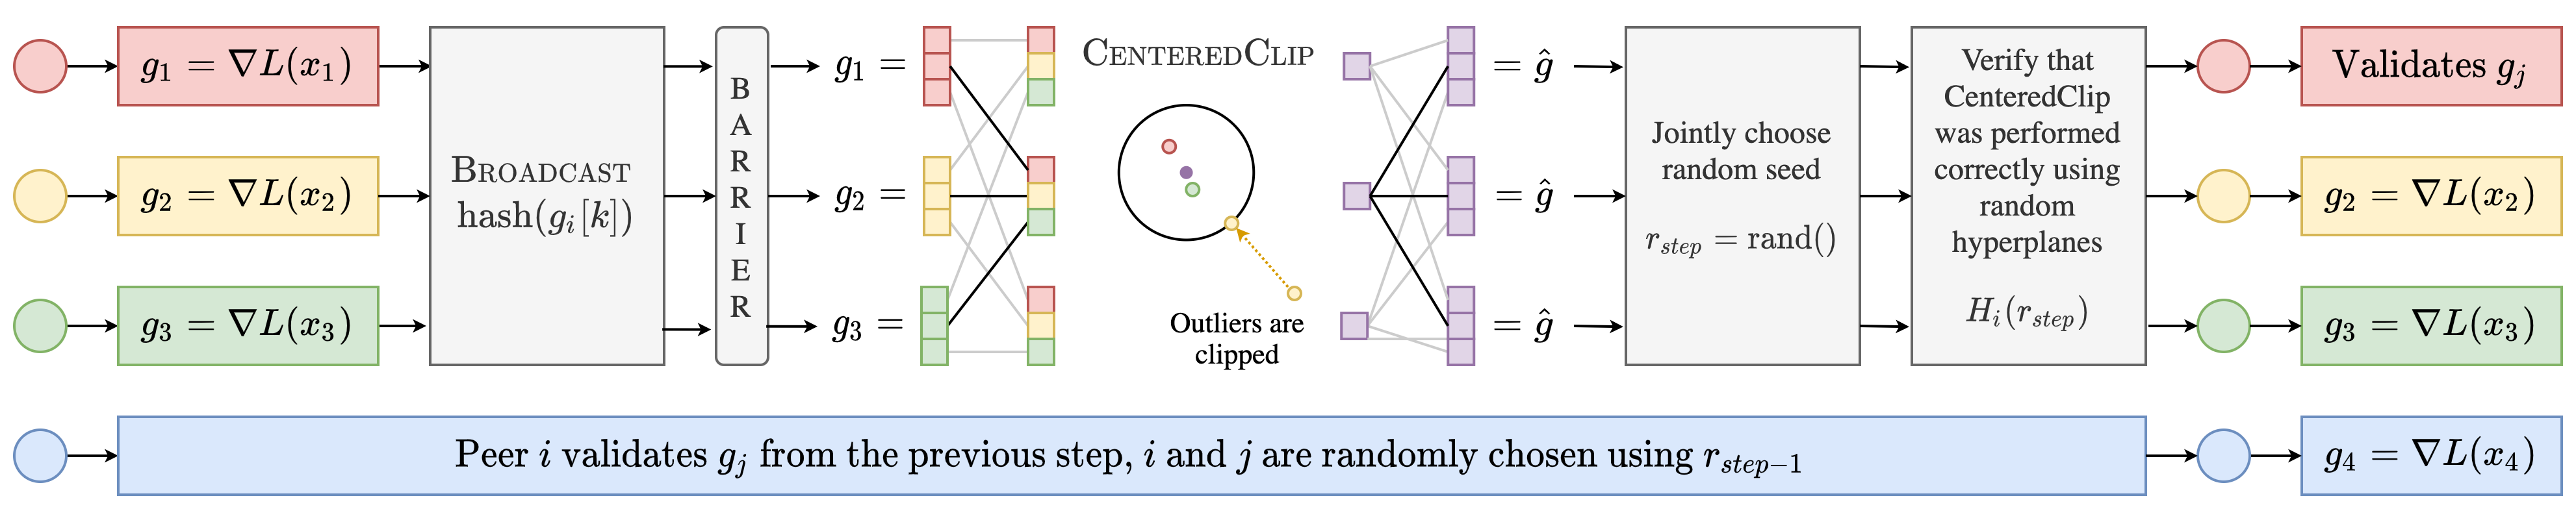
\includegraphics[width=\textwidth]{figs/btard_scheme.png}
\caption{A schematic summary of one step of Byzantine-Tolerant All-Reduce, where $g_i$ are gradients, $r_{\text{step}}$ is the random seed, and $H_i(r_{\text{step}})$ computes the random vector $z$. Image source: \url{https://github.com/yandex-research/btard}.}
\label{fig:BTARD-scheme}
\end{figure}

\section{Experiment}
\label{sec:experiment}

In this project we set out to investigate experimentally the following questions:
\begin{itemize}
    \item How does BTARD-SGD perform on a new learning task, with much fewer parameters?
    \item How does an attack that only perturbs the parameters' values by a small amount perform?
    \item What is the difference in impact between an aggressive attack and a mild attack?
\end{itemize}
\subsection{Experiment design}
\label{sec:experiment-design}
In this project we build on the implementation published with \cite{gorbunov2021secure}, which can be found at \url{https://github.com/yandex-research/btard}, reconfiguring parts of it for simulation on a single physical device. We implement new experiments with BTARD-SGD on a new small convolutional model for MNIST classification, diversifying the model sizes used in its evaluation. This project also contributes two new attacks, \textit{Label Shuffle} and \textit{Noise Addition}, which we evaluate alongside three attacks described in the original BTARD-SGD paper.

Simulating a data-parallel training setup with six workers, we run the following experiments:
\begin{enumerate}[label=\Alph*]
\item The \textit{aggressive} attack: Two Byzantine workers attacking every step, starting at step 100.
\item The \textit{mild} attack: One Byzantine worker attacking every $5^{th}$ step, starting at step 100.
\end{enumerate}

Starting at step 100, in this case, means that the malicious intervention of the Byzantines occurs closer to convergence, even though the simulation runs until 900 steps per experiment. We evaluate BTARD with constant $\tau = 5$, meaning moderate clipping. Each experiment consists of iterating over three different randomly drawn seeds and repeating all runs three times. 

The baseline for comparison will be the same model, trained by the same number of workers in the same configuration, with all workers being honest and non-faulty.

\subsection{Model and learning task}
The model chosen is a simple neural network, with two convolutional layers, each followed by a pooling layer to reduce the parameter space. Its full architecture is depicted in Figure \ref{fig:model}. The loss function is cross-entropy and the optimiser is SGD with Nesterov momentum. The learning rate is scheduled with cosine annealing, with a base learning rate of 0.05. The batch size is 256 per worker and the number of epochs per worker is restricted to four, both selected to lower the total running time of the experiment.

\begin{figure}[h]
\centering
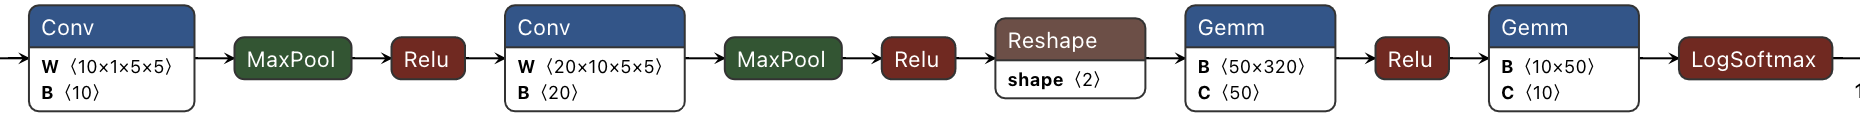
\includegraphics[width=\textwidth]{figs/cnn-shorter.png}
\caption{Visualisation of the convolutional neural network architecture implemented.}
\label{fig:model}
\end{figure}

The model is trained for handwritten digit classification, on the MNIST dataset of handwritten digits \citep{lecun1998gradient, mnist_database}. With 60,000 data points in the training set and 10,000 in the test set, MNIST is a relatively small dataset, allowing for reasonable development iteration times and suitable for simulation in a single GPU environment. %This choice of task, however, limits the merits of a discussion around accuracy values, because even such a small model as the one in Figure \ref{fig:model} achieves $>98\%$ accuracy in as few as two epochs.

\subsection{Restrictions for workers' behaviour}
To best control the simulation and obtain clear results, we make the following system design choices that translate to assumptions about the possible behaviour of the workers:
\begin{enumerate}
    \item All malicious workers start attacking at the same time. 
    \item After a worker is banned, it starts sending correct gradients as if it became a normal peer.
    \item All Byzantine attackers perform the same type of attack.
    \item Byzantine nodes may only \textit{collude} at the beginning and cannot undergo additional malevolent communication later.
\end{enumerate}

The alternative to assumption (2) would have been dropping said worker completely, but that would have posed difficulties in evaluating convergence of the training as the number of replicas would have changed significantly. Additionally, the training data assigned to that node would have to be redistributed or abandoned.

While these restrictions limit how many of the possible attack schemes can be represented through configurations of this implementation, they enable solid simulations both for evaluating the convergence impact of BTARD-SGD and for comparing the different attacks.

\subsection{Attacks}
The types of workers participating in the experiments ran in this project are the following:
\begin{description}
\item \textbf{Normal:} workers compute the cross-entropy loss function for the targets and run the backward pass.
\item \textbf{Amplified Sign Flip:} attackers send the opposite of the true gradient, amplified by 1000 to weigh more in the aggregated gradient if clipping is not used. 
\item \textbf{Amplified Constant Direction Response:} attackers all send large vectors, amplified by 1000, in the same arbitrary direction. The random seed is drawn and passed to all malicious workers just at the start of the training.
\item \textbf{Label Flip:} attackers compute the gradient based on the cross-entropy loss function for flipped labels. Each label value is replaced with $(9 - \text{label})$.
\item \textbf{Label Shuffle:} attackers compute the gradients correctly but pass to the cross-entropy loss function an arbitrary permutation of the targets.
\item \textbf{Noise Addition:} attackers compute the gradients but add random noise to every other parameter $p$ drawn from a Gaussian distribution with $\mu = p$ and $\sigma = 100$.
\end{description}

\textit{Amplified Sign Flip}, \textit{Amplified Constant Direction Response}, and \textit{Label Flip} are used for evaluating BTARD in \cite{gorbunov2021secure}, in their experiments on both ResNet and ALBERT. 
\textit{Label Shuffle} and \textit{Noise Addition} are new attack types developed for this project, which do not appear in the original paper. \textit{Noise Addition} has been introduced to illustrate how a small variation of the parameters impacts the loss and accuracy. This complements attacks such as the \textit{Amplified Constant Direction Response}, which generates parameters that are far away from the mean.

\subsection{System model and setup}

The code is implemented in Python and all dependencies are in the open-source domain. The machine learning framework used is PyTorch, with Netron for the visualisation of the model (Figure \ref{fig:model}) and TensorBoard for visualisation of the results. The NVIDIA CUDA Toolkit is necessary to use Nvidia GPUs for general-purpose computation. The project was run in Google Colab, as it is a simple and effective way to access a CUDA-compatible GPU for small projects. More information about the setup, software dependencies, and decision-making related to the software engineering part of this project is included in the project repository: \url{https://github.com/andreea-zaharia/btard-l46-project}.

The experiment as implemented requires a single GPU, on which it simulates multiple virtual workers as independently spawned processes, using \texttt{torch.multiprocessing}. Each process instantiates a different type of worker that remains the same throughout the training, thus a normal worker cannot suddenly become Byzantine beyond the pre-determined start point of the attack. This is a limitation of the implementation, as it does not account for Byzantine failures due to malfunctioning nodes, but it helps control the simulation and facilitate interpretation of the results. Another limitation introduced by the simulation environment is that the number of workers that can be simulated cannot exceed 6. Thus, to respect the condition that $2f + 1 \leq n$, the number of Byzantine workers cannot exceed 2.

\section{Results}
As we seek to evaluate how the defense behaves on the small model classifying MNIST, a reference point for our analysis is the evaluation presented in \cite{gorbunov2021secure}, where they run experiments on a ResNet architecture for classification on CIFAR-10 and a transformer model, ALBERT. 

In our experiments on the new model, we observe a similar impact on convergence, which supports the merits of the algorithm. The speed of convergence is not worsened but the final accuracy is slightly lower. We will use this drop in accuracy to rank the effectiveness of the individual attacks.

We observe in our experiments a slightly different ranking in the impact of the different attacks presented in the paper, with label flipping being more impactful than sign flipping in both the aggressive and the mild attack schemes. We also find that the newly added attacks have a noticeable impact compared to the baseline, but cause smaller changes in loss and accuracy than the other attacks. This confirms our expectations, as we intended to devise a type of attack performing small magnitude changes. We observe that the algorithm performs well in the presence of these new attacks, too. However, we note a significant negative impact on test accuracy with the aggressive Amplified Constant Direction attack.

The entire experiment took around 1.5 hours on 1x Tesla P100 16GB cloud runtime setup, through Google Colab, with the configuration and the task described in Section \ref{sec:experiment}.

\subsection{The aggressive attack: two Byzantine workers attacking every step}

Figures \ref{fig:learning-curve} and \ref{fig:test-acc} show the loss and accuracy, respectively, for all attacks on this model with the configuration described in Section \ref{sec:experiment-design}. We note that all attacks have a noticeable impact on loss and accuracy as the two Byzantines start their attack in tandem, but BTARD bans all of them quickly and eventually converges to good accuracy on the MNIST task.

\begin{figure}[h!]
\centering
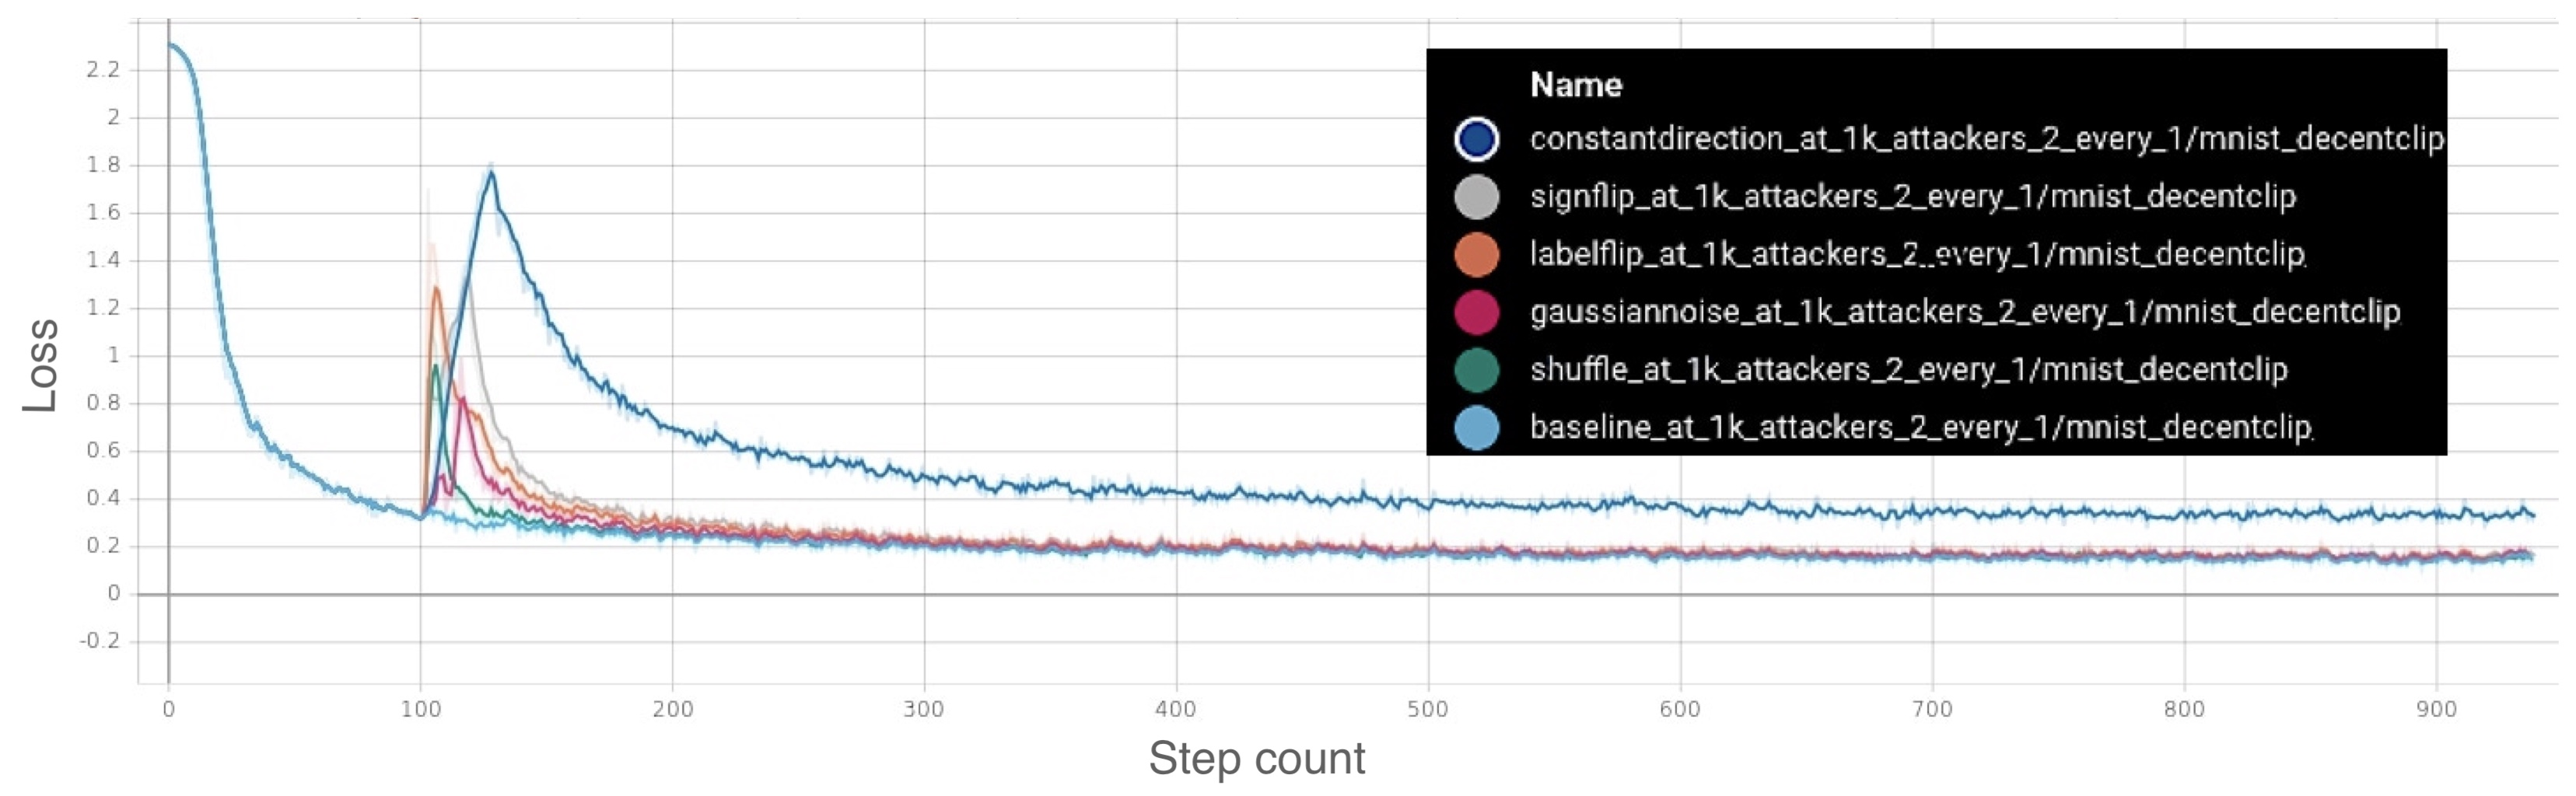
\includegraphics[width=\textwidth]{figs/aggressive_attack_loss.jpg}
\caption{Learning curves of the loss function for BTARD-SGD with moderate clipping. All attacks. Training with 6 workers, including two Byzantines starting to attack at step 100.}
\label{fig:learning-curve}
\end{figure}

On this model, the \textit{Amplified Constant Direction Response} attack has the most significant impact. The training still converges, but at the end of the training, at the $900^{th}$ step, the test accuracy remains over 0.01 below all the others. For the MNIST classification task, this is a notable difference. The other attacks have only a minor negative impact on convergence, which can be reasonably discussed as negligible.
% \begin{figure}
% \centering
% \includegraphics[width=\textwidth]{figs/train_loss_all_2every1.jpeg}
% \caption{Learning curves with all attacks. 6 workers, including 2 Byzantines starting to attack at the  step.}
% \label{fig:learning-curve-zoom}
% \end{figure}

\begin{figure}[h!]
\centering
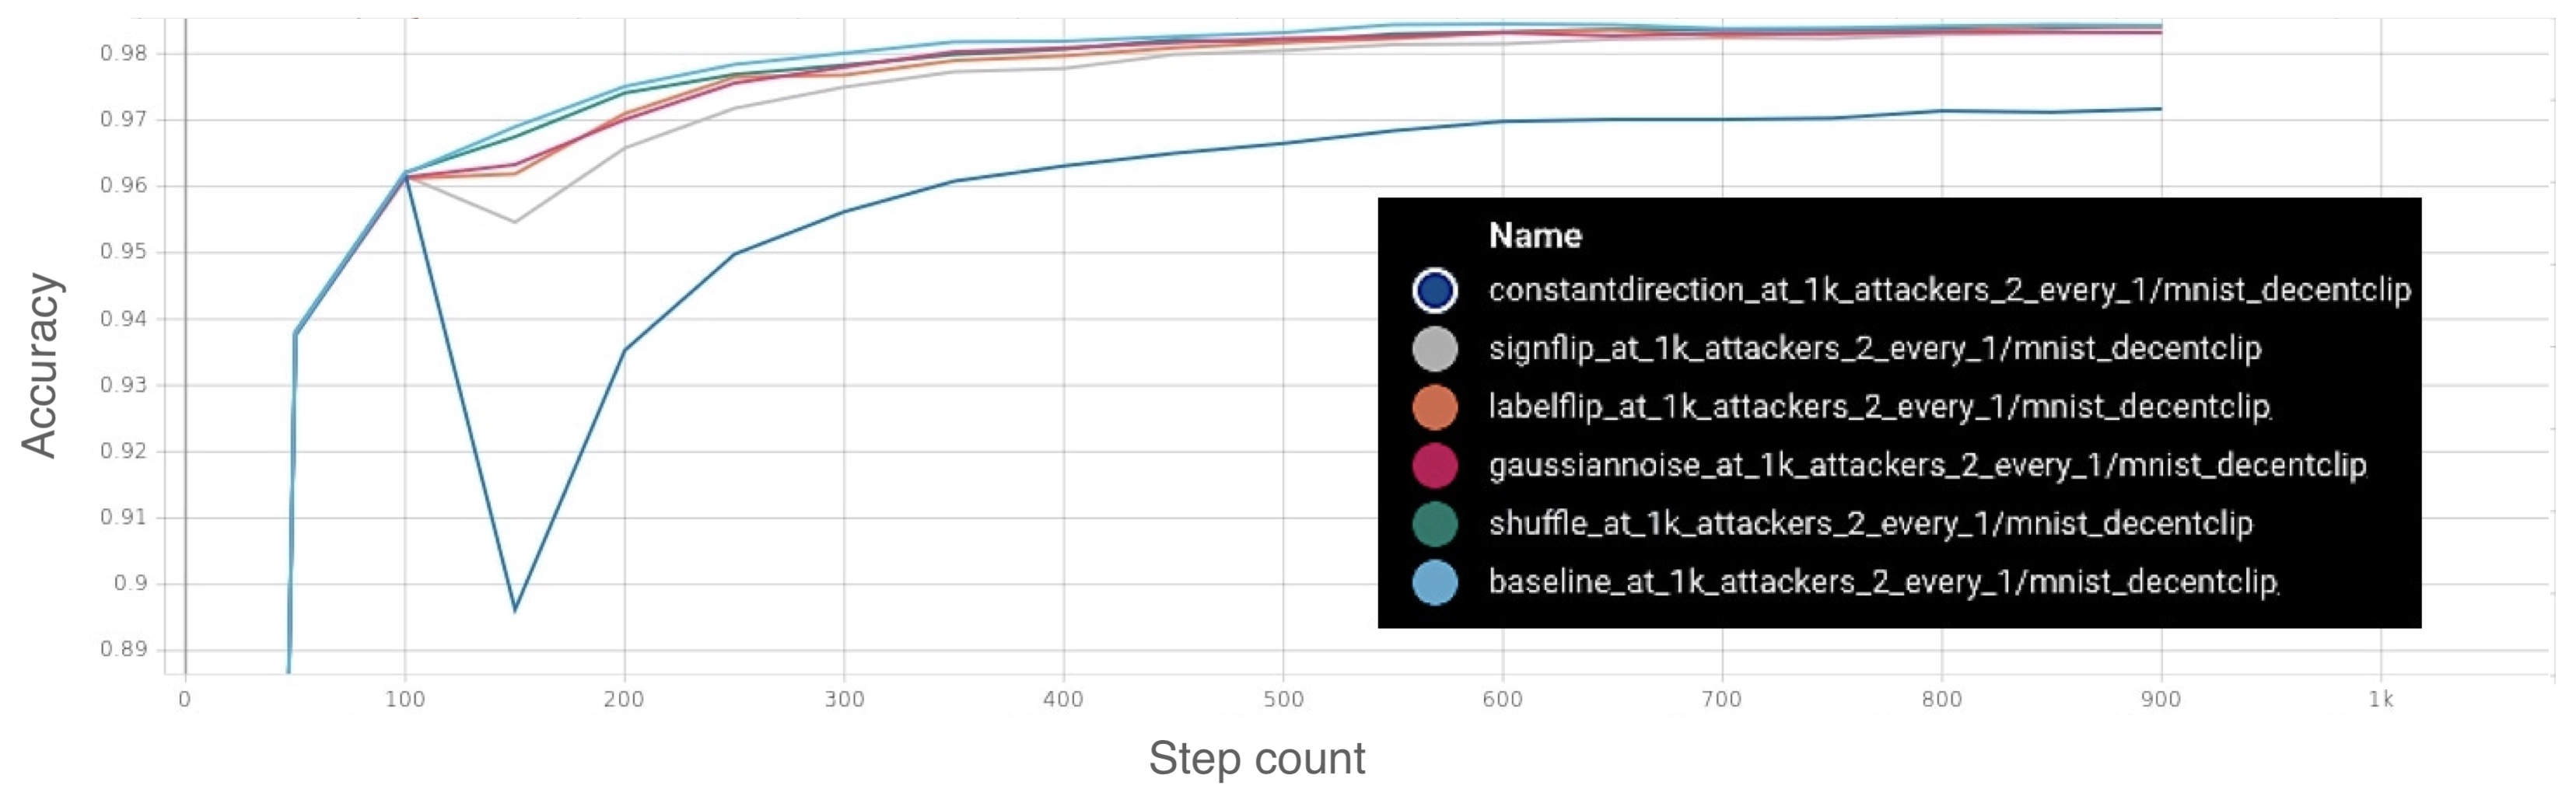
\includegraphics[width=\textwidth]{figs/aggressive_attack_accuracy.jpeg}
\caption{Test accuracy for BTARD-SGD with moderate clipping. All attacks. Training with 6 workers, including two Byzantines starting to attack at step 100.}
\label{fig:test-acc}
\end{figure}

\subsection{The mild attack: one Byzantine worker attacking every five steps}
In the mild attack, the attack strategies do not stray far from the baseline, being nearly indistinguishable from noise other than at the attack start step and soon after. For both loss (Figure \ref{fig:learning-curve-mild}) and accuracy (Figure \ref{fig:test-acc-mild}) we note the higher magnitude impact of the \textit{Amplified Constant Direction Response} attack, but this time its course is corrected towards convergence, preventing it from yielding a drop in test accuracy at the end of training.
\begin{figure}[h!]
\centering
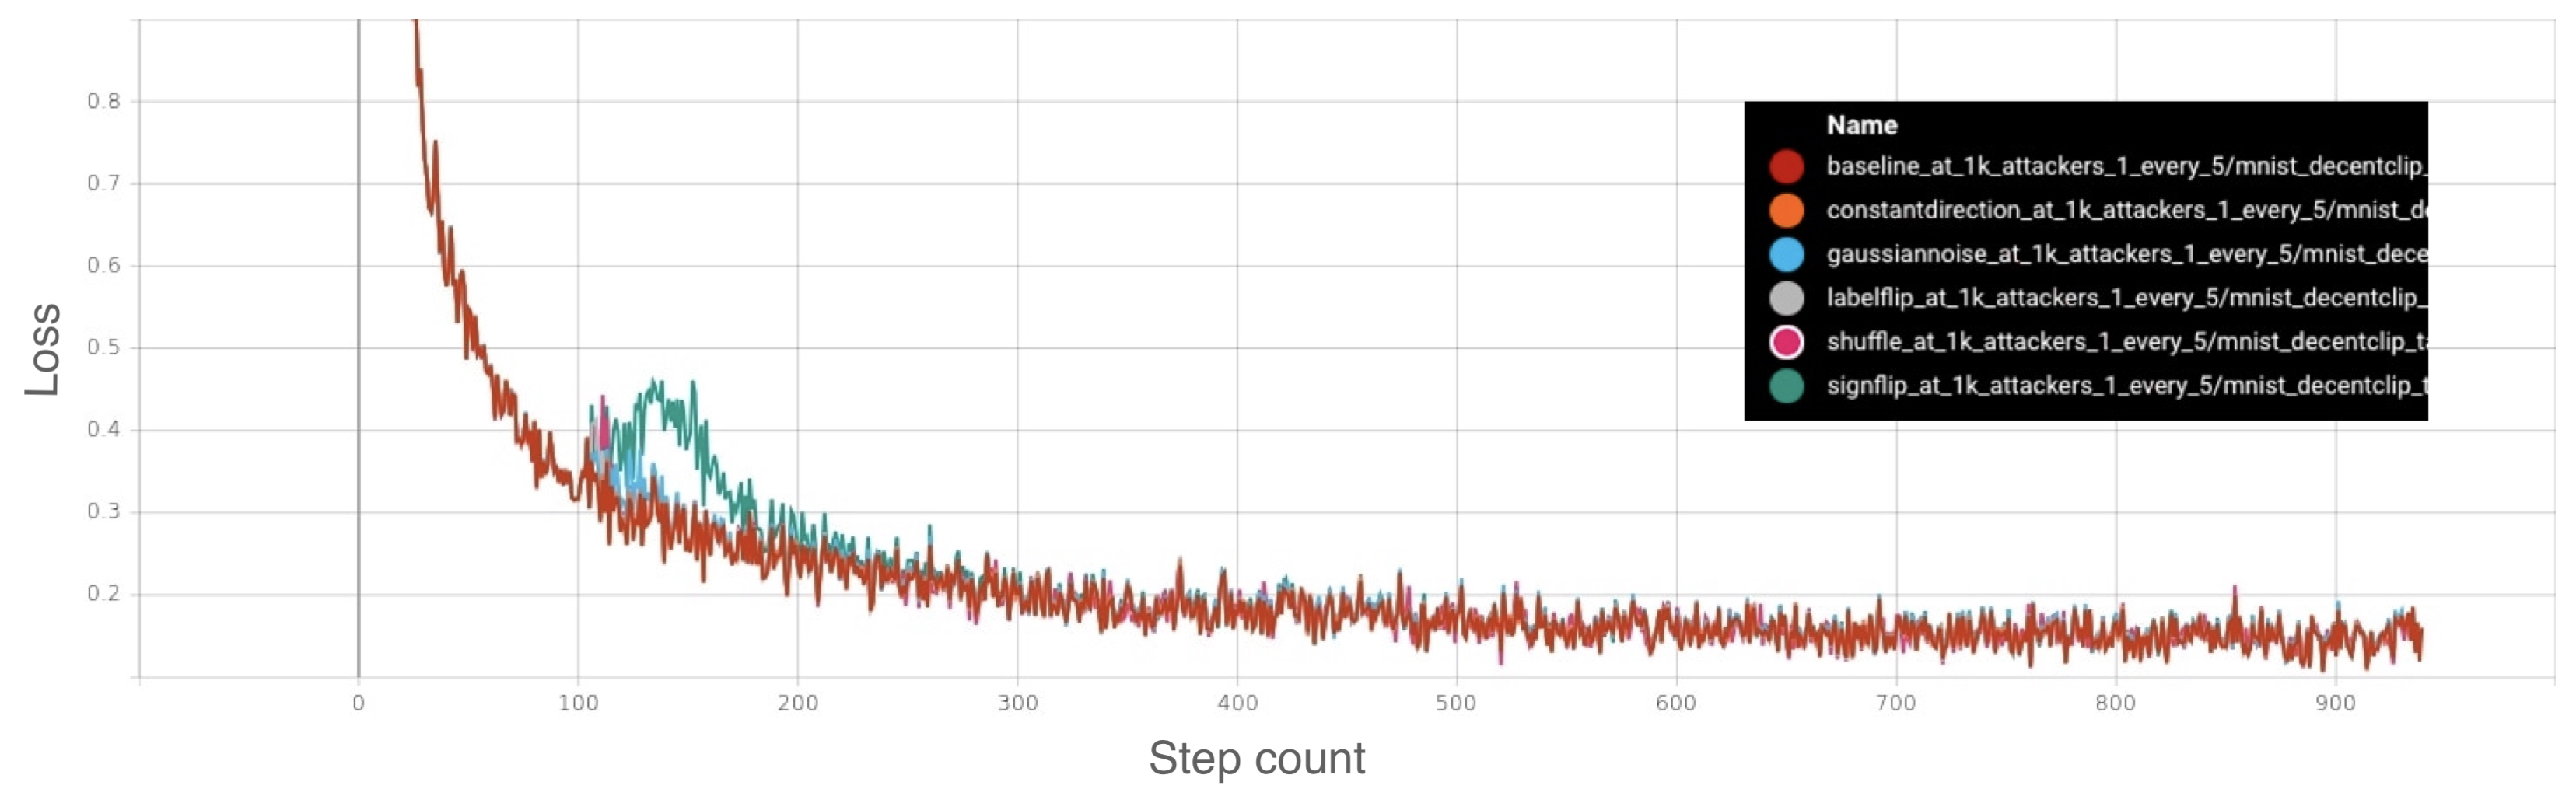
\includegraphics[width=\textwidth]{figs/mild_attack_loss_zoomed_in.jpg}
\caption{Learning curves of the loss function for BTARD with moderate clipping, zoomed in. All attacks. Training with 6 workers, including a Byzantine attacking every fifth step, starting at step 100.}
\label{fig:learning-curve-mild}
\end{figure}

\begin{figure}[h!]
\centering
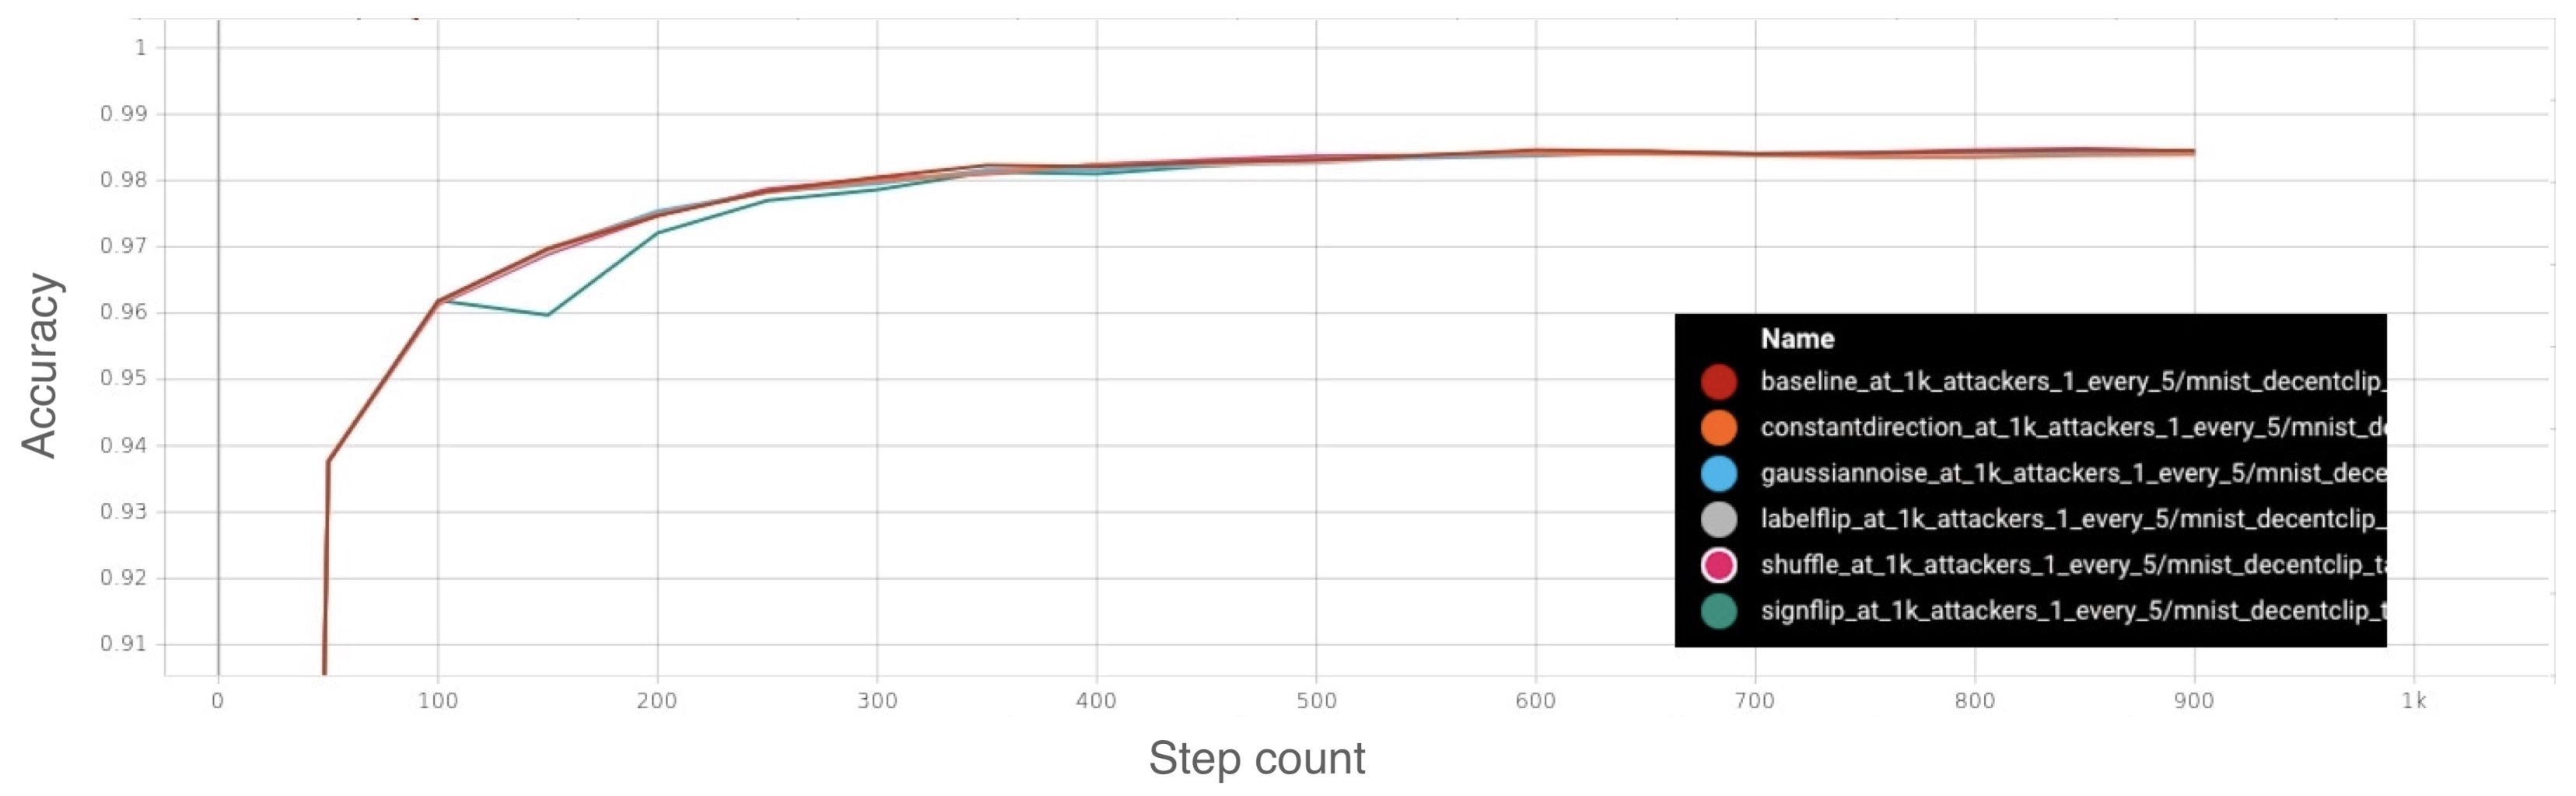
\includegraphics[width=\textwidth]{figs/mild_attack_accuracy.jpg}
\caption{Test accuracy for BTARD-SGD with moderate clipping, zoomed in. All attacks. Training with 6 workers, including a Byzantine attacking every fifth step, starting at step 100.}
\label{fig:test-acc-mild}
\end{figure}

\section{Directions for future work}

Directions for future work could cover an investigation into how violating individual assumptions alters the convergence in practice, such as by decoupling the start times across attackers and combining attackers of different types in the same experiment. A related project could also examine the performance of Butterfly Clip in the presence of aggregation attacks, which were set outside the scope of this project. Extending to an actual multi-GPU setup would allow larger-scale experiments for a greater variety of attack schemes with the same, or more, attacker types.

\section{Conclusion}
This project investigated Byzantine attacks and defenses in data-parallel distributed training, with public datasets. We evaluate Byzantine-Tolerant All-Reduce Stochastic Gradient Descent, proposed by \cite{gorbunov2021secure}, on a new model and learning task, introducing new gradient attacks employed by Byzantine workers, in a controlled simulation environment. The conclusions we draw are largely in agreement with the experiments in the original paper, with minor differences that do not affect the correctness or scalability of the algorithm. Lastly, BTARD-SGD succeeds in banning the attackers employing the new attack strategies introduced, \textit{Label Shuffle} and \textit{Noise Addition}.

\bibliographystyle{plainnat}
\bibliography{biblio}

\end{document}